\documentclass[12pt,a4paper]{ctexart}

\usepackage[UTF8]{ctex}
\usepackage{geometry}
\usepackage{graphicx}
\usepackage{xcolor}
\usepackage{tikz}
\usepackage{fontspec}
\usepackage{setspace}
\usepackage{enumitem}
\usepackage{booktabs}
\usepackage{array}
\usepackage{longtable}
\usepackage{hyperref}
\usepackage{fancyhdr}
\usepackage{titlesec}
\usepackage{multicol}
\usepackage{xurl}
\usepackage{tocloft}

\renewcommand{\cfttoctitlefont}{\hfill\bfseries\Large}
\renewcommand{\cftaftertoctitle}{\hfill}
\geometry{left=2.5cm,right=2.5cm,top=2.5cm,bottom=2.5cm}

\definecolor{black}{RGB}{0,0,0}
\definecolor{mainblue}{RGB}{0,82,147}
\definecolor{accentgold}{RGB}{180,140,60}
\definecolor{lightgray}{RGB}{245,245,245}
\definecolor{darkgray}{RGB}{80,80,80}
\definecolor{mainred}{RGB}{230,1,45}

\hypersetup{
    colorlinks=true,
    linkcolor=black,
    urlcolor=mainblue,
    citecolor=mainblue,
    pdfborder={0 0 0}
}

\pagestyle{fancy}
\fancyhf{}
\fancyhead[L]{\small\color{darkgray}\textbf{量子行业每周新闻洞察}}
\fancyhead[R]{\small\color{darkgray}\textbf{总第183期}}
\fancyfoot[C]{\thepage}
\renewcommand{\headrulewidth}{0.4pt}
\renewcommand{\footrulewidth}{0pt}

\titleformat{\section}
    {\Large\bfseries\color{mainred}}
    {\thesection、}{0em}{}
\titleformat{\subsection}
    {\large\bfseries\color{mainred}}
    {\thesubsection、}{0em}{}

\newcolumntype{L}[1]{>{\raggedright\arraybackslash}p{#1}}
\newcolumntype{C}[1]{>{\centering\arraybackslash}p{#1}}

\begin{document}

% ==================== 封面 ====================
\begin{titlepage}
\begin{tikzpicture}[remember picture,overlay]
    \fill[mainred] ([yshift=-0.5cm]current page.north west) rectangle ([yshift=-1.2cm]current page.north east);
    \fill[mainred] ([yshift=1.2cm]current page.south west) rectangle ([yshift=0.5cm]current page.south east);
\end{tikzpicture}

\vspace*{4cm}

\begin{center}
    {\fontsize{44}{52}\selectfont\bfseries\color{black} \textbf{量子行业每周新闻洞察}}

    \vspace{0.8cm}

    {\fontsize{16}{22}\selectfont\color{darkgray} 2026.06.06 — 2026.06.12 }
    {\fontsize{16}{22}\selectfont\color{darkgray} \textbf{WEEKLY NEWS}}

    \vspace{1.5cm}

    {\fontsize{20}{26}\selectfont\color{mainred}\textbf{（总第\textbf{ 183 }期）}}

    \vspace{4cm}

    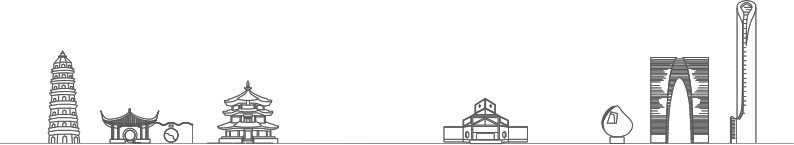
\includegraphics[width=\textwidth]{Cover_Suzhou.png}

    \vfill

    {\fontsize{12}{16}\selectfont\color{darkgray} 量子科技长三角产业创新中心\\编制：战略情报与成果专利室、产业发展部（理事会办公室）}
\end{center}
\end{titlepage}

% ==================== 目录 ====================
\pagenumbering{roman}
\newpage
\tableofcontents

\newpage

% ==================== 摘要 ====================
\pagenumbering{arabic}
\setcounter{page}{1}
\begin{center}
{\Large\bfseries\color{mainred} 摘\hspace{2em}要}
\end{center}
\addcontentsline{toc}{section}{摘要}


\textbf{ 宏观态势：}

全球量子科技竞争正从单点突破转向体系化布局与跨国协同。各国政府通过设立专门委员会、签署双边协议及启动联合项目，加速构建量子通信与计算领域的战略联盟。美日达成迄今规模最大的10亿美元科研合作，德波捷三国启动QUANT-GPlCz量子密钥分发网络，印度与德国两度会晤聚焦量子卫星通信，显示技术主权与标准制定成为博弈焦点。产业界巨头日立与英特尔在量子计算等五大领域展开协作，Classiq携手智利天主教大学开拓拉美首个量子计算病理学研究。但与此同时，英国白皮书警示资金、人才与政府采购等结构性挑战仍存，产业长期健康发展需政策持续发力。


\textbf{ 科技前沿：}

基础研究与工程实现正合力突破量子系统的核心瓶颈。超导量子计算领域，中科大团队首次在双层镍氧化物中观测到无节点超导能隙与电子-玻色子耦合，IQM发布"杠铃码"使逻辑错误率降低三个数量级，新南威尔士大学借鉴"薛定谔猫"开发出高效纠错新方法，共同推动容错量子计算迈向实用化。量子光源方面，台湾清华研发出全球最亮单光子源（每秒23亿颗光子），南洋理工开发出水中仍保持高亮度的新型量子点。拓扑与二维材料研究中，南科大高振团队在手性束缚态与三维光学量子霍尔效应上连获突破，上海交大在多层石墨烯中发现新奇量子物态，南开团队实现拓扑磁结构的飞秒激光操控。此外，预测代理框架将量子处理器测量开销降低超99.97\%，港大极低温神经形态硬件为量子计算规模扩展提供新路径，EPFL成功将超快激光器集成到光子芯片上，标志着量子技术平台正走向更高集成度与复杂度。


\textbf{ 产品动态：}

量子技术产品正从实验室样机加速迈向工业级应用与系统集成。量子安全领域出现实质性突破，Quantropi与诺基亚联合推出的一体化密钥分发方案已完成真实环境测试，微软在Windows 11与Server 2025系统中深度集成后量子密码功能，从网络层到操作系统层筑牢抗量子安全防线。计算硬件方面，Rigetti 108量子比特处理器正式上线Amazon Braket云平台，大阪大学推出全球首个量子多编程自动模式提升云吞吐量。值得关注的是，AI与量子计算交叉融合趋势凸显——微软利用智能体AI显著缩短Majorana 2芯片实验周期，伯克利国家实验室MODMD混合框架以极低资源需求实现分子能量状态计算。新加坡国立大学开发出目前最高安全等级的QRNG芯片，是德科技ADS光子设计器新增对格芯硅光子工艺支持，显示专用模块与开发生态日趋成熟。


\textbf{ 企业资讯：}

产业生态建设呈现技术纵深整合与多方协同攻关的鲜明态势。Quantum X Labs与IQCC合作评估AI量子纠错算法，OQC联合摩根大通和AMD探索量子-AI融合金融服务应用，Yaqumo、NKT Photonics与滨松光子签署备忘录构建冷原子量子计算光学供应链，反映出产业链各环节正加速协同。组织发展层面，Diraq任命CMOS领域资深领袖McGregor为新任董事会主席，悉尼大学量子团队成立研究型公司Emergence Quantum补全技术"缺失环节"，伊利诺伊量子产业园和魁北克PINQ2分别强化技术领导力与学术合作，高校成果转化与企业战略布局并行推进，量子产业生态在人才汇聚与跨界合作中持续完善。


\textbf{ 资本运作：}

资本正以重仓之势涌入量子赛道，推动产业进入高估值、大额融资与公开市场并行的新阶段。头部量子计算公司Quantinuum以16.8亿美元完成IPO，IQM SPAC上市获SEC批准即将登陆纳斯达克，标志行业逐步走向公开市场。国内本源量子以210亿元估值完成近30亿元Pre-IPO轮融资，创下国内量子企业估值新高；中国电信联合国盾量子设立15亿元产业投资基金，彰显国资对量子生态的系统级布局。产业链上游成为投资热点，禾信仪器3.84亿元跨界收购量羲技术进军稀释制冷机赛道，武汉超磁科技完成天使轮融资推动超导磁体国产化，QTREX获以色列创新署资助开发专用介电材料，SEALSQ收购Miraex补齐量子互连关键环节。英国2000万英镑资助量子优势加速器项目，澳大利亚QuantX Labs获种子轮融资，政府引导与市场资本共同为量子软硬件研发注入强劲动能。




\textbf{ 专利动态：}

本周专利动态涵盖超导量子测控技术、量子软件与算法、量子算力网、量子科技长三角产业创新中心共4个板块、17条专利。




% ==================== 会议列表 ====================
{
    \newpage
    \section*{ 6月量子科技行业国内、国际会议}
    \addcontentsline{toc}{section}{ 6月量子科技行业国内、国际会议}
    \scriptsize
    \begin{longtable}{C{0.8cm}L{2.5cm}L{3cm}L{7cm}}
        \toprule[1.5pt]
        \textbf{序号} & \textbf{日期} & \textbf{地点} & \textbf{会议名称} \\
        \midrule
        \endfirsthead
        \toprule
        \textbf{序号} & \textbf{日期} & \textbf{地点} & \textbf{会议名称} \\
        \midrule
        \endhead
        \bottomrule
        \endfoot
        
        1 & 6月1日-3日 & 拉勒米, 美国 & 第四届怀俄明大学量子暑期学校 \\
        \midrule[0.05pt]
        
        2 & 6月1日-5日 & 罗利, 美国 & 2026量子机器学习暑期研讨会 \\
        \midrule[0.05pt]
        
        3 & 6月1日-5日 & 普罗维登斯, 美国 & 第57届APS原子、分子与光物理年会 \\
        \midrule[0.05pt]
        
        4 & 6月2日-4日 & 特隆赫姆, 挪威 & 量子自旋电子学 \\
        \midrule[0.05pt]
        
        5 & 6月3日-4日 & 罗切斯特, 美国 & 量子热力学与退相干 \\
        \midrule[0.05pt]
        
        6 & 6月4日-5日 & 东京, 日本 & Q2B：量子价值路线图 \\
        \midrule[0.05pt]
        
        7 & 6月5日 & 格拉斯哥, 英国 & 量子与社会研究研讨沙盒 \\
        \midrule[0.05pt]
        
        8 & 6月7日-12日 & 圣巴巴拉, 美国 & 第八届国际量子纠错会议 \\
        \midrule[0.05pt]
        
        9 & 6月7日-13日 & 克里特岛, 希腊 & 青年原子光学会议 \\
        \midrule[0.05pt]
        
        10 & 6月8日-11日 & 滑铁卢, 加拿大 & 量子光子学 \\
        \midrule[0.05pt]
        
        11 & 6月8日-20日 & 卡尔热斯, 法国 & 量子技术计算与通信暑期学校 \\
        \midrule[0.05pt]
        
        12 & 6月8日-8月14日 & 洛斯阿拉莫斯, 美国 & 2026洛斯阿拉莫斯量子计算暑期学校 \\
        \midrule[0.05pt]
        
        13 & 6月9日 & 巴黎, 法国 & Q-Day量子风险峰会：后量子密码学与量子密钥分发 \\
        \midrule[0.05pt]
        
        14 & 6月10日-12日 & 华沙, 波兰 & Perspektywy科技女性峰会 \\
        \midrule[0.05pt]
        
        15 & 6月10日-12日 & 多恩比恩, 奥地利 & 第四届砷化镓量子点国际研讨会 \\
        \midrule[0.05pt]
        
        16 & 6月10日-12日 & 埃朗根, 德国 & 神经形态计算前沿 \\
        \midrule[0.05pt]
        
        17 & 6月11日 & 杰克逊维尔, 美国 & 量子当下，医疗未来 \\
        \midrule[0.05pt]
        
        18 & 6月15日-17日 & 苏黎世, 瑞士 & 欧洲集成光学会议（ECIO） \\
        \midrule[0.05pt]
        
        19 & 6月15日-18日 & 格拉斯哥, 英国 & Optica Quantum 2.0会议 \\
        \midrule[0.05pt]
        
        20 & 6月15日-18日 & 赫尔辛基, 芬兰 & 仲夏开放量子系统、退相干及量子-经典交叉会议 \\
        \midrule[0.05pt]
        
        21 & 6月15日-18日 & 洛杉矶, 美国 & 量子器件设计研讨会 \\
        \midrule[0.05pt]
        
        22 & 6月16日 & 巴黎, 法国 & 第5届France Quantum \\
        \midrule[0.05pt]
        
        23 & 6月16日-17日 & 伦敦, 英国 & 第5届年度量子商业化全球大会2026 \\
        \midrule[0.05pt]
        
        24 & 6月16日-17日 & 格拉斯哥, 英国 & Optica 2026量子产业峰会——第5届 \\
        \midrule[0.05pt]
        
        25 & 6月21日-25日 & 塞费尔德, 奥地利 & 第57届欧洲原子系统组年度会议（EGAS 57） \\
        \midrule[0.05pt]
        
        26 & 6月21日-26日 & 塞费尔德, 奥地利 & 第7届塞费尔德量子信息研讨会 \\
        \midrule[0.05pt]
        
        27 & 6月21日-7月4日 & 贝纳斯克, 西班牙 & 量子科学：实现 \\
        \midrule[0.05pt]
        
        28 & 6月22日-24日 & 奥斯陆, 挪威 & IQT北欧：变化世界中的量子技术 \\
        \midrule[0.05pt]
        
        29 & 6月26日 & 汉堡, 德国 & 第7届ISC HPC国际研讨会——监控、可观测性与运营数据分析 \\
        \midrule[0.05pt]
        
        30 & 6月26日 & 汉堡, 德国 & 第2届统一计算中心量子资源研讨会（QRUCH） \\
        \midrule[0.05pt]
        
        31 & 6月26日 & 汉堡, 德国 & 第5届量子及混合量子/经典计算方法研讨会 \\
        \midrule[0.05pt]
        
        32 & 6月26日 & 汉堡, 德国 & 科学与工业数字孪生研讨会——从数据科学家到数据中心 \\
        \midrule[0.05pt]
        
        33 & 6月22日-7月3日 & 雷苏什, 法国 & 2026光子与原子暑期学校：量子气体、光-物质相互作用、量子技术 \\
        \midrule[0.05pt]
        
        34 & 6月23日-24日 & 罗马(纽约州), 美国 & 量子国际年度研讨会（Q4I） \\
        \midrule[0.05pt]
        
        35 & 6月23日-26日 & 阿尔加维, 葡萄牙 & 第3届量子安全网络与系统研讨会（QSNS 2026） \\
        \midrule[0.05pt]
        
        36 & 6月25日-26日 & 波士顿, 美国 & Quantum.Tech World \\
        \midrule[0.05pt]
        
        37 & 6月29日-7月1日 & 汉堡, 德国 & 国际计算科学大会量子计算专题 \\
        \midrule[0.05pt]
        
        38 & 6月29日-7月3日 & 贝桑松, 法国 & 第14届欧洲频率与时间研讨会（EFTS） \\
        \midrule[0.05pt]
        
        39 & 6月29日-7月10日 & 阿斯巴雷拉斯, 西班牙 & La Ricotta暑期学校：干草堆中的量子 \\
        \midrule[0.05pt]
        
        40 & 6月30日-7月1日 & 柏林, 德国 & GITEX欧洲 \\
        \midrule[0.05pt]
        
    \end{longtable}
}




% ==================== 宏观态势 ====================
\newpage
\section{宏观态势}
\vspace{-0.5em}
\noindent\rule{\linewidth}{1.5pt}

\subsection{ 得克萨斯州州长任命五位专家加入该州的量子计划咨询委员会 }

2026年06月09日消息，美国得克萨斯州州长Greg Abbott近日宣布任命五位专家加入该州的“量子计划咨询委员会”，以推动得克萨斯州的量子经济发展。其中，Victor Fishman博士与Lin Zhou博士的任期至2027年1月31日，Richard·Ross·Coffman任期至2029年1月31日，John Josephakis与Jeff Prevost博士任期至2031年1月31日。该委员会将负责制定战略规划，并促进得州量子产业生态建设。

\noindent\textbf{报道链接：}\url{https://gov.texas.gov/news/post/governor-abbott-appoints-five-to-quantum-initiative-advisory-committee}

\subsection{ 德国图林根州长访问印度，两国将在量子通信与光子学技术领域展开合作 }

2026年06月09日消息，印度与德国近日就量子通信、光子学、量子卫星通信、空间技术和深科技创新等领域探讨了如何建立面向未来的合作伙伴关系。德国图林根州州长Mario Voigt访印期间，与印度科技国务部长Jitendra Singh会晤，双方围绕量子网络、光学地面站、先进光子技术及科研产业协同展开了交流。印度方面还介绍了其国家量子任务进展，包括安全量子通信及相关技术的突破。此外，双方还就量子计算、量子通信及配套基础设施的发展交换了意见。

\noindent\textbf{报道链接：}\url{https://www.indiablooms.com/news/india-and-germany-explore-deep-tech-partnership-in-quantum-space-and-advanced-technologies/details}

\subsection{ 印度与德国将加速深科技领域的合作，量子卫星通信成双方焦点 }

2026年06月10日消息，印度和德国在量子通信领域的合作近日迎来重要进展。两国的高级别官员已在新德里举行会谈，重点探讨了在量子通信、光子学、太空技术及其他前沿深科技领域的合作。印度科技部表示，此次会谈凸显了先进技术在推动创新、经济增长及两国战略合作中的日益重要作用。双方还就扩大量子卫星通信合作进行了深入交流。

\noindent\textbf{报道链接：}\url{https://indianmasterminds.com/news/government/india-germany-quantum-communication-space-deep-tech-cooperation-2026-208087/}

\subsection{ 美日斥资10亿美元达成规模最大科研合作之一，聚焦量子科技等六大领域 }

2026年06月10日消息，美国能源部（DOE）与日本文部科学省、日本经济产业省近日宣布建立一项价值10亿美元（未来五年内各投入5亿美元）的战略合作伙伴关系，使日本成为特朗普总统“创世使命”的首个国际合作伙伴。这是美日两国间迄今规模最大、意义最为深远的科学与技术合作之一。根据协议，十一个联合科研团队将联合12家DOE国家实验室、一处DOE科学办公室用户设施以及日本12家顶尖研究机构，汇聚全球最先进的科研设施、计算资源与人才，共同推动量子信息科学、聚变能源、生物技术、先进材料、粒子物理及自主实验室系统等领域的突破。

\noindent\textbf{报道链接：}\url{https://www.energy.gov/articles/united-states-and-japan-announce-historic-1-billion-partnership-under-president-trumps}

\subsection{ 德波捷三国携手推进量子密钥分发技术，QUANT-GPlCz项目正式启动 }

2026年6月，德国-波兰-捷克量子密钥分发网络项目QUANT-GPlCz启动，由EuroQCI倡议资助，欧盟和德国联邦数字化和现代化部（BMDS）平等支持。项目由诺德豪森应用技术大学协调，弗劳恩霍夫IOF、HHI、IIS、柏林工业大学、慕尼黑工业大学、DE-CIX和耶拿量子光学有限公司参与，旨在连接德波捷三国量子通信骨干网，连接法兰克福、柏林、华沙、布拉格，并整合德国Q‑net‑Q、波兰PIONIER‑Q和捷克CZQCI网络。项目将测试数据中心高安全性互连、关键基础设施和政府通信保护方案，并实现地面光纤与空间段的耦合。

\noindent\textbf{报道链接：}\url{https://www.squad-germany.de/en/launch-of-trilateral-qkd-infrastructure-project/}

\subsection{ 新发布的报告认为英国量子产业面临资金、人才与采购支持等关键挑战 }

2026年06月09日消息，一份最新白皮书警告称，尽管英国已在量子技术领域投入超过10亿英镑的公共资金并占据早期全球领先地位，但若不采取更强有力的措施支持规模化融资、人才培养、供应链建设、政府采购和研究资助，该国可能难以捕捉长期经济价值。该报告指出，后期成长资本短缺、劳动力挑战以及政府对量子技术的采购有限，是实现英国到2033年占据全球量子市场15\%份额并吸引相应私人投资目标的关键障碍。此外，该报告还呼吁加大对量子网络的投资、重新评估量子安全方面的政策信号，并继续支持基础研究，以避免削弱支撑英国量子产业发展的科学根基。

\noindent\textbf{报道链接：}\url{https://thequantuminsider.com/2026/06/04/uk-risks-repeating-semiconductor-and-ai-mistakes-unless-government-acts-now-on-quantum-warns-cross-party-parliamentary-group/}

\subsection{ 日立与英特尔达成战略合作，将在量子计算等五大核心领域展开协作 }

2026年06月08日消息，日立公司与英特尔公司近日宣布建立战略合作关系，将在制造、能源、出行等关键行业共同探索物理人工智能、先进计算及下一代数字基础设施的应用机遇。双方计划围绕五大战略支柱——晶圆代工工具、量子计算、能源优化、定制芯片与边缘AI应用、工厂自动化——展开协作，以开发新解决方案并优化现有流程。这其中，在量子计算领域，双方研发团队将加强联合开发，加速量子技术进步并创造新价值。

\noindent\textbf{报道链接：}\url{https://www.hitachi.com/en/press/articles/2026/06/0605/}

\subsection{ 智利天主教大学与Classiq携手，探索利用混合量子算法革新生物医学图像分析 }

2026年06月08日消息，Classiq与智利天主教大学近日宣布启动一项联合研究项目，旨在利用经典机器学习及英伟达CUDA-Q量子-经典计算平台，开发用于生物医学图像分析的混合量子算法。这项为期12个月、名为“通过量子计算增强病理学”的合作，由智利天主教大学资助。这是拉丁美洲首个将量子计算、机器学习与计算病理学相结合的公开联盟。项目初期聚焦肾脏病理学，具体研究包括将量子机器学习应用于计算病理学，重点攻关肾脏病变分类、肾小球自动分割以及全组织病理切片的语义模式搜索。该研究将借助Classiq量子计算软件平台与英伟达CUDA-Q平台，实现从算法开发到模拟与执行的无缝工作流。

\noindent\textbf{报道链接：}\url{https://www.globenewswire.com/news-release/2026/06/04/3307069/0/en/classiq-and-uc-chile-launch-quantum-ai-research-for-biomedical-image-analysis-leveraging-integration-with-nvidia-cuda-q.html}


% ==================== 科技前沿 ====================
\newpage
\section{科技前沿}
\vspace{-0.5em}
\noindent\rule{\linewidth}{1.5pt}

\subsection{ 我国学者在镍基高温超导机理研究取得进展 }

中国科学技术大学何俊峰研究组与南方科技大学薛其坤-陈卓昱团队，首次在Ruddlesden‑Popper相双层镍氧化物高温超导薄膜中，直接观测到无节点超导能隙与电子‑玻色子耦合现象，成果发表于Science。团队利用高分辨率ARPES，在(La,Pr,Sm)3Ni2O7薄膜中测得约18 meV稳定无节点超导能隙，表明更接近s波对称性；并在费米能级下约70 meV处观测到“能带扭折”，确认了电子-玻色子耦合的存在。

\noindent\textbf{报道链接：}\url{https://www.science.org/doi/10.1126/science.adw8329}

\subsection{ 每秒23亿颗光子台湾清华大学研发出全球最亮量子光源 }

台湾清华大学材料系林皓武团队在室温下打造出全球最亮高速不闪烁单光子源，每秒发射超23亿颗光子，成果发表于Science Advances。团队使用“两性离子”配体包覆钙钛矿量子点，使其能嵌入约10奈米的银奈米立方体“电浆子奈米共振腔”中，产生帕塞尔效应，发光速度提升435倍、强度增加250倍，发光效率达95\%。

\noindent\textbf{报道链接：}\url{https://www.science.org/doi/10.1126/sciadv.aec4380}

\subsection{ 国际科研团队在一种半导体材料中观测到激子与声子的相干“量子舞蹈” }

2026年06月11日消息，一个国际研究团队最近观测到了半导体材料中激子与声子共同演化而形成的完全相干量子舞蹈。通常情况下，晶格振动会迅速破坏脆弱的量子态，但研究者在卤化铅钙钛矿纳米晶体中发现了例外：在2开尔文的低温下，晶格振动保持稳定，使得量子态可相干演化约10皮秒。该团队利用超短激光脉冲直接追踪了这一演化过程，并观察到激子与晶格振动能量交换产生的显著量子拍频。结果证明，通过简单改变纳米晶体尺寸即可调控该效应，这为设计和控制该系统的量子动力学开辟了一条实用途径。相关成果已于日前在《自然·通讯》上发表。

\noindent\textbf{报道链接：}\url{https://www.eurekalert.org/news-releases/1131480}

\subsection{ IQM发布“杠铃码”：逻辑错误率降低三个数量级，物理比特需求骤降八倍 }

2026年06月11日消息，IQM量子计算机公司近日宣布开发出一种新型量子纠错码“barbell codes（杠铃码）”，可将逻辑错误率比表面码降低三个数量级，同时所需物理量子比特数最多减少八倍。该纠错码属于量子低密度奇偶校验（qLDPC）码家族，专为IQM“星座”系统独特的量子处理器拓扑结构而设计。与许多高性能量子纠错方案不同，该新码保持了较低的硬件复杂度，为可扩展容错量子计算迈出重要一步。

\noindent\textbf{报道链接：}\url{https://iqm.tech/press-releases/iqm-announces-novel-quantum-error-correction-approach-toward-fault-tolerant-quantum-computing/}

\subsection{ 上海交大陈国瑞课题组首个混合堆垛多层石墨烯量子物态的系列实验研究取得重要进展 }

上海交通大学物理与天文学院陈国瑞课题组首次制备高质量混合堆垛五层石墨烯器件，相关成果发表于Nano Letters和Nature Communications。研究揭示了ABCBC五层石墨烯的内禀层极化，观测到多重Lifshitz转变，并在极低温强磁场下发现电场可调的偶数分母分数量子霍尔态，如v=-5/2、-7/2等。

\noindent\textbf{报道链接：}\url{https://pubs.acs.org/doi/full/10.1021/acs.nanolett.6c01016}

\subsection{ 深圳国际量子研究院李正达课题组在多方量子非定域性研究方面取得重要进展 }

深圳量子研究院李正达课题组将Gisin两体非局域性定理推广至多体系统，首次在多拷贝网络框架下证明所有多体纯态的全局真正纠缠与全局真正非定域性等价，成果发表于Physical Review Letters。实验上，团队在传统Svetlichny不等式无法判定的参数区间内，成功验证了三体GHZ类和W类态的全局真正量子非定域性。

\noindent\textbf{报道链接：}\url{https://journals.aps.org/prl/abstract/10.1103/mwxx-ln9v}

\subsection{ 碳纳米带中的量子磁性与拓扑设计 }

英国巴斯大学物理系Michele Pizzochero博士在Nano Letters发表研究，通过在富勒烯纳米带边缘添加一个富勒烯分子，在非磁性材料中创造出自旋-1/2中心，可排列成反铁磁链。另一项研究展示了通过纳米带边缘特定原子排列产生手性电子态，为构建拓扑电子态提供了自下而上的方法。

\noindent\textbf{报道链接：}\url{https://www.bath.ac.uk/announcements/designing-quantum-magnetism-and-topology-in-carbon-nanoribbons/}

\subsection{ 新研究表明经物理训练的数字“超级大脑”可加速光学元件开发 }

瑞典查尔姆斯理工大学Philippe Tassin团队在Laser \& Photonics Reviews发表研究，通过向神经网络内置电磁学物理定律，将纳米光子学设计所需的数据训练时间缩短至原来的十分之一。该超级大脑能加速人工光学材料模拟，用于量子计算机的光传输和相机镜片等领域。

\noindent\textbf{报道链接：}\url{https://www.chalmers.se/en/current/news/fa-physics-trained-digital-super-brain-speeds-up-technology-development/}

\subsection{ 武汉大学于霆教授团队利用二维磁性半导体CrSBr实现“自旋调制发光器件” }

武汉大学物理科学与技术学院于霆团队在Nature Communications发表研究，创新性采用CrSBr量子阱结构，成功制备出集成二维磁性半导体的自旋调制发光器件。当电子自旋翻转时，发光强度出现阶跃式突变；自旋倾斜时，发光能量和强度可实现连续线性可调。

\noindent\textbf{报道链接：}\url{https://doi.org/10.1038/s41467-026-71489-7}

\subsection{ 南科大高振课题组首次在自偏置磁光光子晶体中实验实现磁诱导手性连续域束缚态 }

南方科技大学电子与电气工程系高振课题组在PNAS发表研究，首次在自偏置磁光光子晶体中实验观测到手性连续域中的束缚态（chiral BICs）。该体系基于镧掺杂钡铁氧体（La:BaM），无需外加磁场，通过剩余磁化强度打破时间反演对称性，使简并BICs劈裂为一对手性相反的BICs。

\noindent\textbf{报道链接：}\url{https://www.pnas.org/doi/10.1073/pnas.2536341123}

\subsection{ 南开团队在新型拓扑磁结构领域取得重要进展 }

南开大学物理科学学院付学文团队在Advanced Materials发表研究，依托自研4D超快透射电子显微镜，在中心对称二维范德华磁体Cr1.6Ti0.03Te2中实现飞秒激光对多种新型偶

\noindent\textbf{报道链接：}\url{https://advanced.onlinelibrary.wiley.com/doi/10.1002/adma.73589}

\subsection{ 科学家开发的预测代理计算框架能学习并复现量子处理器的输出结果 }

2026年06月09日消息，河南省量子信息与量子密码重点实验室和新加坡南洋理工大学的研究人员合作开发了一种称为预测代理的新型计算模型，能够学习并复现量子处理器的输出结果。该框架的核心优势在于其严格的理论保障：只需使用从量子处理器收集的相对少量数据完成训练，预测代理就能够在经典计算端预测大量后续计算的结果。在验证性任务中，他们将其应用于变分量子本征求解器的优化加速以及非平衡量子物质相的识别。结果显示，预测代理在这两类任务中均实现了高预测精度，同时将测量开销降低了超过99.97\%。相关研究成果已于日前发表在《自然·通讯》期刊。

\noindent\textbf{报道链接：}\url{https://phys.org/news/2026-06-surrogates-quantum-overhead.html}

\subsection{ 科学家在菱面体石墨烯中发现异常超导态，有望推动量子技术发展 }

2026年06月10日消息，有佛罗里达州立大学物理学家参与的一项国际合作研究发现，菱面体石墨烯中会出现异常的超导态，有望驱动意想不到的量子技术的发展。相关研究已于日前发表在《自然物理》杂志上。在这个由几层碳原子堆叠组成的系统中，电子几乎完全局域在材料的顶层和底层表面，而材料内部的体态电荷极少，且超导性正是直接源于这种双表面构型，其中电子和空穴载流子协同作用形成超导态。除了超导性，该团队还观测到量子反常霍尔效应。研究人员表示，如果超导行为与拓扑态最终能实现共存，理论上将出现马约拉纳零模，这可能成为容错量子计算的基石构建块。

\noindent\textbf{报道链接：}\url{https://news.fsu.edu/news/science-technology/2026/06/08/collaborative-research-by-fsu-physicists-uncovers-novel-electronic-properties-in-quantum-material/}

\subsection{ 港大团队开发出极低温神经形态硬件，有望为量子计算规模扩展提供新路径 }

2026年06月10日消息，香港大学工程学院电机与计算机工程系与先进半导体与积体电路研究中心（CASIC）的研究人员，近日在低温电子学领域取得重大突破。他们开发出一款可在接近绝对零度下运行的可编程神经形态硬件平台，为扩展量子计算规模及实现深空探测提供了潜在解决方案。这一研究的意义在于，它为超导量子计算机的关键外围控制电路提供了一种基于传统半导体材料的低功耗、可扩展方案，有望突破当前量子比特数量扩展的瓶颈。相关研究成果已于日前发表在《自然·通讯》上。

\noindent\textbf{报道链接：}\url{https://www.hku.hk/press/news\_detail\_29161.html}

\subsection{ 台湾大学研究人员展示通过界面工程实现无电压调控两种材料间的电子空间排布 }

2026年06月10日消息，近日，台湾大学的研究人员在《自然·通讯》发表了一项新研究，展示了如何通过界面工程，在半金属铋（Bi）薄膜与二维半导体二硫化钼（MoS2）之间实现电子空间排布的双向精确控制，且无需施加任何电压。由于该材料系统无需外部电压即可实现电子约束，它为开发电荷量子比特和超低功耗器件提供了关键基础，有望为下一代量子计算和节能半导体芯片开辟新的设计路径。

\noindent\textbf{报道链接：}\url{https://www.asiaresearchnews.com/content/bidirectional-manipulation-gate-free-quantum-electronic-states-semiconductor-device}

\subsection{ 南洋理工大学科学家开发出新型量子点技术，能在极低浓度下保持高亮度 }

2026年06月10日消息，新加坡南洋理工大学的科学家开发出一种新型钙钛矿纳米晶体（即量子点），其在水环境中仍能保持高亮度和稳定性。该团队创新性地将原本用于保护纳米晶体表面的铵卤化物分子重新利用，以推动一种在水中形成双层保护壳的工艺。处理后，能使纳米晶体在水中既能保持分散和稳定，即使在极低浓度下仍保持高亮度，能重新发射出所吸收光线的80\%。这一成果有望推动量子技术和生物成像领域的发展。

\noindent\textbf{报道链接：}\url{https://www.ntu.edu.sg/research/research-hub/news/detail/lighting-a-bright-future-for-quantum-technology-by-keeping-water-out}

\subsection{ 科学家开发的新型二维金属有机框架能解决堆叠二维材料导致的性能下降瓶颈 }

2026年06月10日消息，韩国科学技术院（KAIST）的研究团队成功开发出一种新的二维导电金属有机框架（MOF），其即使在多层堆叠状态下也能保持单层电子特性。 该研究发现，这种材料在保持高导电性的同时，能最大限度减少层间干扰，即使在多层状态下，该材料仍能保留与单层高度相似的电子结构，尤其是支持电子快速高效移动的狄拉克能带结构（Kagome晶格特性）。这一成果突破了长期以来多层二维材料层间效应影响性能的瓶颈，为新型量子器件和电子设备的开发提供了关键材料基础。

\noindent\textbf{报道链接：}\url{https://news.kaist.ac.kr/newsen/html/news/?mode=V\&mng\_no=62730\&skey=category\&sval=research\&list\_s\_date=\&list\_e\_date=\&GotoPage=1}

\subsection{ 北京量子院超快光谱学团队在激子极化激元弛豫机制研究中取得重要进展 }

2026年06月08日消息，近日，北京量子信息科学研究院（以下简称“量子院”）超快光谱学团队在单层WS
2
微腔激子极化激元弛豫机制研究中取得重要进展，揭示了温度、激发功率和腔失谐对极化激元弛豫的协同调控作用，为理解二维TMDs微腔极化激元动力学及高性能器件设计提供了新思路。2026年3月17日，相关成果以“单层WS 2 微腔中激子极化激元弛豫的微观机制”（Microscopic Mechanisms of Exciton Polariton Relaxation in Monolayer WS 2 Microcavities）为题，发表于《ACS 纳米》（ACS Nano）。

\noindent\textbf{报道链接：}\url{https://pubs.acs.org/doi/abs/10.1021/acsnano.5c18736}

\subsection{ 北京量子院陆全勇团队与合作者在中红外微腔光频梳研究方面取得重要进展 }

2026年06月09日消息，近日，北京量子信息科学研究院（以下简称“量子院”）陆全勇团队与中国科学院半导体研究所刘峰奇、张锦川团队合作，在中红外微腔光频梳研究方面取得重要进展，首次提出并实现了一种工作在室温条件下的中红外定向辐射微腔量子级联激光器（QCL）光学频率梳，成功解决了传统环形微腔光源光提取效率低、定向发射能力差等难题，为中红外光频梳光谱学及亚太赫兹通信提供了一个极具前景的高性能单片集成平台。2026年5月26日，相关成果以“基于量子级联激光器的破缺型微腔光频梳”（Notched microcomb based on a quantum-cascade laser）为题，发表在《光学》（
Optica
）上。


\noindent\textbf{报道链接：}\url{https://doi.org/10.1364/OPTICA.585839}

\subsection{ 中国科学院精密测量院在量子纠缠加速生成方面取得重要进展 }

2026年06月09日消息，近日，中国科学院精密测量院冯芒研究团队与郑州大学等单位合作，在囚禁离子实验平台首次实现了非厄米体系中纠缠生成的加速，成功超越传统厄米量子速度极限，将纠缠态制备速度提升了1.52倍。该研究成果于2026年5月28日在线发表在《物理评论快报》（Physical Review Letters）上。

\noindent\textbf{报道链接：}\url{https://journals.aps.org/prl/abstract/10.1103/g8v5-rbq7}

\subsection{ EPFL成功将超快激光器集成到光子芯片 性能可与台式飞秒激光器媲美 }

2026年06月08日消息，本文内容全由AI翻译，仅供参考
2026年6月3日——超快激光器发射的脉冲仅持续几百飞秒，即千万亿分之一秒。这些光脉冲为从精密微加工、眼科手术到光学频率梳等应用提供动力，而后者的诺贝尔奖技术正是当今最精确光学原子钟的基础。然而，尽管经过二十多年的努力，超快激光器在很大程度上仍然是笨重、昂贵的系统，被局限在光学实验台上。
如今，由EPFL的Tobias J. Kippenberg教授领导的团队已将其集成到光子芯片上。研究人员在《自然》杂志上报告了首款集成超快激光器，其性能可与台式飞秒激光器相媲美，可在短至147飞秒的脉冲中提供1.05纳焦耳的能量。

\noindent\textbf{报道链接：}\url{https://actu.epfl.ch/news/a-ultrafast-laser-on-a-chip-4/}

\subsection{ 挪威科学家利用新理论研究解释了为什么光子无法一分为二 }

2026年06月09日消息，挪威奥斯陆大学的一个研究团队发现，试图将一个光子一分为二并不会产生两个更小的光子，而是会凭空创造出无限多个光子。在该研究中，他们设想了一个实验场景：让一个单光子通过一个可快速开关的光学快门（本质上是超高速反射镜），以阻挡部分光脉冲。结果显示，快门并未在阻挡侧产生真空，反而生成了一个包含无限多光子态的叠加态。这一现象源于量子力学中的“真空不空”，即量子力学空间利充满了电磁场的量子涨落。快速切换快门会扰动这些涨落，从而自发创造出新光子。该理论研究已于近日发表在《物理评论快报》杂志。

\noindent\textbf{报道链接：}\url{https://phys.org/news/2026-06-photon-infinite-swarm-particles.html}

\subsection{ 弗吉尼亚联邦大学科学家在量子计算小型化方面取得重要进展 }

2026年06月07日消息，本文内容全由AI翻译，仅供参考
2026年6月3日——量子计算曾一度仅存在于理论可能性中，它有望带来更快、更节能的计算机——但这需要科学家们能够构建并规模化运行这些机器所需的硬件。弗吉尼亚联邦大学的新研究让科学家们向实用规模的量子计算迈进了一小步，这有望显著降低某些行业的能耗和计算时间。
在这项近期发表于《自然通讯》的研究中，研究人员利用比光波长小两倍的微型磁体，构建了量子计算的基本模块，开创了一项技术，可能减少打造可实用量子计算机所需的物理空间。


\noindent\textbf{报道链接：}\url{https://news.vcu.edu/article/vcu-researchers-advance-quantum-computing-with-tiny-virus-sized-nanomagnets}

\subsection{ 中国科大通过晶体对称性破缺实现闪锌矿量子点定向发光 }

2026年06月08日消息，近日，中国科学技术大学自旋磁共振实验室樊逢佳教授团队与河南大学申怀彬教授、曾在平教授、王垒副教授团队合作，在量子点定向发光研究中取得重要进展。研究团队首次发现，通过在闪锌矿量子点中引入堆垛层错，可以打破其原有晶体对称性，使传统上被认为难以实现取向发光的准球形闪锌矿量子点产生高效定向发光。相关成果以“Crystalline symmetry breaking enables directional light emission in quantum dots”为题，发表于国际学术期刊《自然·光子学》（Nature Photonics）。


\noindent\textbf{报道链接：}\url{https://www.nature.com/articles/s41566-026-01935-x}

\subsection{ 南科大高振团队首次实验实现费米弧三维光学量子霍尔效应 }

2026年06月08日消息，近日，南方科技大学电子与电气工程系高振副教授团队首次在时间反演对称性破缺的三维非均匀磁性外尔光子晶体中实验实现了费米弧三维光学量子霍尔效应并直接观测到其典型特征-单侧手性棱态。相关成果以“Three-dimensional photonic quantum Hall effect of Fermi arcs”为题发表在National Science Review上。


\noindent\textbf{报道链接：}\url{https://academic.oup.com/nsr/advance-article/doi/10.1093/nsr/nwag251/8665134}

\subsection{ 芝加哥大学研究人员提出能简单创建高度复杂纠缠量子态的新方法 }

2026年06月08日消息，芝加哥大学普利兹克分子工程学院的研究人员提出一种生成高度复杂纠缠量子态的简化理论方法，相关成果已于日前发表在《物理评论X》上。传统上，产生此类深层次纠缠态需要复杂工具与精心设计的装置，但该团队发现，利用量子物理实验室中通用的腔量子电动力学装置，只需调整不同原子的能量分配，即可创建并控制多种纠缠状态。研究人员表示，该方法可直接应用于超精密量子传感技术，用于探测两地微小磁场或引力差异，对基础物理研究也具有重要意义。

\noindent\textbf{报道链接：}\url{https://pme.uchicago.edu/news/researchers-craft-new-simple-recipe-highly-entangled-quantum-states}

\subsection{ 法国量子计算公司Alice \& Bob发布五条标准框架以评估逻辑量子比特性能 }

2026年06月08日消息，法国量子计算公司Alice \& Bob近日发布了一个具有五项标准的评估框架，旨在为逻辑量子比特提供定义与性能基准，以建立跨硬件模态的公平且全面的性能评价体系。这五项评估标准是：盈亏平衡点、可扩展参数、足够的量子纠错周期、全运行性能和实用时间尺度。该框架可帮助投资者、分析师、企业决策者及研究人员客观比较不同性能、成熟度与能力水平的硬件成果，它提供了一个简单的清单，可以将与容错量子计算（FTQC）相关的进展与较弱的演示区分开来。

\noindent\textbf{报道链接：}\url{https://www.hpcwire.com/off-the-wire/alice-bob-proposes-five-criteria-framework-for-evaluating-logical-qubits/}

\subsection{ 德国科学家发现了稠密里德堡气体与超冷等离子体间的微观联系 }

2026年06月08日消息，德国汉堡大学的一个研究团队近日在《Communications Physics》上发表新研究，证明通过调节超快激发过程中产生的电子初始能量，可以系统地探索稠密里德堡气体向超冷等离子体的转变过程，并为这一转变提供了统一的微观描述。在该研究中，团队通过调节激发电子的初始能量，追踪了自由电子、离子与里德堡原子之间的平衡演化。先进的数值模拟结果与测量数据在定量上高度吻合，为该实验发现提供了有力支持。实验和模拟共同表明，相同的微观框架可以描述不同激发状态下高密度里德堡气体中超冷等离子体的产生。

\noindent\textbf{报道链接：}\url{https://www.cui-advanced.uni-hamburg.de/en/research/wissenschaftsnews/26-06-05-rydberg-gas.html}

\subsection{ 塔斯基吉大学研发出新型量子发射器，有望推动下一代量子技术发展 }

2026年06月08日消息，塔斯基吉大学材料科学系的研究人员最近在量子材料领域取得进展，他们开发出一种基于金属氧化物的新型量子发射器，有望加速下一代量子计算、通信和传感技术的发展。在该研究中，团队利用一种简单、可扩展的微波合成技术，成功制备出一类新型多孔锰钴铁氧体纳米颗粒，为量子器件的实际集成开辟了新路径。

\noindent\textbf{报道链接：}\url{http://tuskegee.edu/news/2026/06/Tuskegee-University-Scientists-Achieve-Breakthrough-in-Quantum-Materials.html}

\subsection{ 新南威尔士大学借助“薛定谔猫”灵感开发出高效量子纠错新方法 }

2026年06月07日消息，新南威尔士大学悉尼分校的工程师们借鉴了著名的“薛定谔的猫”类比，提出了一种更高效的方法，用于消除量子计算中的错误。

“想象一下，在黑暗嘈杂的房间里，你的猫藏在八个一模一样的纸箱中的一个里，” 新南威尔士大学Scientia教授Andrea Morello说，“你不允许进入房间——打开门可能会害死猫。那么，找到它藏在哪里的最佳策略是什么？我们的量子研究团队找到了这个问题的答案，这可能是构建量子计算机道路上的一个重要里程碑。”
几十年来，这个猫的比喻一直被用来阐释将量子力学应用于宏观系统时出现的奇异现象。

在这项由新南威尔士大学主导的研究中，“猫”是植入硅量子芯片的一个锑原子核。尽管原子尺度很小，但这个锑核拥有八个量子态，可用于编码量子信息。
拥有八个不同的状态为检测和纠正计算过程中可能出现的错误留下了额外的空间。


\noindent\textbf{报道链接：}\url{https://www.unsw.edu.au/newsroom/news/2026/06/dont-scare-the-cat-engineers-find-smarter-way-to-measure-quantum-systems}


% ==================== 产品动态 ====================
\newpage
\section{产品动态}
\vspace{-0.5em}
\noindent\rule{\linewidth}{1.5pt}

\subsection{ Quantropi与诺基亚联手推出量子安全密钥分发一体化方案，已完成真实环境测试 }

2026年06月11日消息，量子安全技术公司Quantropi近日宣布，与诺基亚联合推出一款可实现规模化量子安全密钥分发的一体化解决方案。该方案将Quantropi的数字量子密钥分发技术与诺基亚的安全管理服务器相结合，能为关键网络提供具备抗量子能力的带外密钥分发。目前，该联合解决方案已在Numana的量子通信测试平台Kirq上成功部署，验证了其在真实环境下的性能、互操作性及大规模部署的成熟度。

\noindent\textbf{报道链接：}\url{https://www.prnewswire.com/news-releases/quantropi-announces-general-availability-of-integrated-nokia-solution-delivering-quantum-safe-outofband-key-distribution-302794566.html}

\subsection{ 日本研究团队首创性地开发出量子多编程自动模式，可大幅提升系统吞吐量 }

2026年06月11日消息，日本大阪大学量子信息与量子生物学中心（QIQB）联合系统工程顾问公司及顺天堂大学的研究人员，近日在其量子计算云服务中，上线了全球首个量子多编程自动模式。该功能可自动将不同用户的量子程序并行运行于同一量子处理器，从而减少闲置量子比特资源、提升系统吞吐量，从而实现缓解量子云计算的拥堵问题。此前发布的量子多编程手动模式仅支持同一用户手动指定多个程序并行执行，而新自动模式能从云队列中筛选合适任务，分配给可用量子比特并同步执行。这项新功能不仅仅是填充芯片上的空白空间，它还利用了数学优化来确定如何高效地布局多个量子电路。

\noindent\textbf{报道链接：}\url{https://qiqb.osaka-u.ac.jp/en/newstopics/pr20260609}

\subsection{ 新加坡国立大学开发出目前具有最高安全等级的量子随机数生成器芯片 }

2026年06月11日消息，新加坡国立大学的一个研究团队开发出一种具备自检功能的量子随机数生成器（QRNG）芯片。该芯片在QRNG芯片中实现了迄今为止最高的安全等级，其安全分析假设对手可能与探测器本身存在量子关联这一最坏情况。它会在运行过程中实时验证自身测量硬件的完整性，即使在面对具备量子计算能力的攻击者时，其安全性依然有保障。相关研究成果已于日前发表在《PRX Quantum》上。

\noindent\textbf{报道链接：}\url{https://cde.nus.edu.sg/news/nus-cde-researchers-develop-self-testing-quantum-chip-for-digital-security/}


\subsection{ Rigetti的108量子比特处理器在Amazon Braket平台上线 }

2026年06月09日消息，亚马逊AWS近日宣布，Rigetti的108量子比特超导量子处理单元Cepheus-1-108Q现已正式在其Amazon Braket平台上线。这是该平台首个百比特以上门型量子设备，它取代了之前的Rigetti Ankaa-3系统。该物理设备位于美国，能提供7*20小时的量子任务处理可用性。据了解，该处理器采用Rigetti专有的多芯片架构，将12个9量子比特小芯片拼接成单个处理器，其中值双量子比特门保真度达到了99.1\%，门操作速度约为60纳秒。

\noindent\textbf{报道链接：}\url{https://aws.amazon.com/cn/blogs/quantum-computing/amazon-braket-launches-rigetti-cepheus-1-108q-superconducting-device/}

\subsection{ 微软已在Windows 11与Server 2025系统中支持后量子密码学功能 }

2026年06月09日消息，微软近日为Windows 11与Windows Server 2025扩展了后量子密码学能力，重点应对“先窃取、后解密”带来的长期数据安全风险。此次更新不再局限于算法和开发接口，而是进一步覆盖系统协议与企业基础设施。目前，Windows TLS协议栈加入了量子安全混合密钥交换，Windows密码学API中则支持了混合PQC算法，Active Directory证书服务也可签发后量子证书。微软称，这将帮助企业逐步评估并迁移现有PKI与通信安全体系。

\noindent\textbf{报道链接：}\url{https://techcommunity.microsoft.com/blog/microsoft-security-blog/new-windows-features-to-secure-today\%E2\%80\%99s-data-in-a-post-quantum-world/4523370?utm\_source=chatgpt.com}


\subsection{ 微软已利用AI智能体助力研发Majorana 2芯片，显著缩短实验周期 }

2026年06月09日消息，微软正将智能体AI全面融入其量子计算项目，以加速Majorana 2芯片的开发、实现研究工作流程自动化，并助力其在2029年前建成一台商用级量子计算机。该公司表示，AI智能体可协助科学家分析近二十年的研究数据，识别跨学科的模式，管理复杂的工程依赖关系，并发现可能被忽视的制造问题。微软称，通过自动化测量、优化材料研究，并让研究人员更高效地测试和改进量子器件设计，智能体AI已能显著缩短实验周期。

\noindent\textbf{报道链接：}\url{https://thequantuminsider.com/2026/06/03/ai-powered-quantum-microsoft-turns-to-agentic-ai-to-speed-quantum-computing-push/}

\subsection{ 是德科技ADS光子设计器新增对格芯硅光子工艺技术的支持 }

2026年06月08日消息，Keysight（是德科技）近日宣布，其先进设计系统（ADS）光子设计器已新增对GlobalFoundries（格芯）硅光子工艺技术的支持，从而扩大了其光子集成电路（PIC）开发代工生态系统。设计人员现在可以在单一环境中，从PIC设计直接过渡到完整的电-光-电（EOE）系统仿真，以在流片前验证光子电路在光链路层面的性能。是德科技表示，这套面向ADS光子设计器的格芯CLO PDK现已上市。

\noindent\textbf{报道链接：}\url{https://www.keysight.com/us/en/about/newsroom/news-releases/2026/0603\_pr26-075-keysight-expands-photonics-design-ecosystem-with-globalfoundries-pdk.html}

\subsection{ 伯克利国家实验室开发的混合框架MODMD能以低资源需求揭示分子能量状态 }

2026年06月08日消息，美国劳伦斯伯克利国家实验室的研究人员开发出一种名为多观测动态模式分解（MODMD）的高效混合框架，通过将简化的量子“快照”与经典数据分析相结合，能大幅降低计算资源需求，使当前早期量子计算机得以探索复杂分子的能量状态。该框架利用流体动力学中的数据分析和高效量子测量策略，能以极少的计算能力实现快速且误差可控的分析，可同时计算量子系统的基态和激发态能量，从而获取光谱与动力学信息，为揭示分子行为本质铺平道路。

\noindent\textbf{报道链接：}\url{https://cs.lbl.gov/news-and-events/news/2026/new-hybrid-approach-bypasses-hardware-limits-to-unlock-complex-quantum-simulations/}



% ==================== 专利动态 ====================
\newpage
\section{专利动态}
\vspace{-0.5em}
\noindent\rule{\linewidth}{1.5pt}

\subsection{ 超导量子测控技术 }

\subsubsection{ 一种行波微波光量子探测方法、系统及一种超导量子电路 }

申请人：深圳市永达电子信息股份有限公司

发明人：戚建淮 | 王明帅 | 胡金华 | 王胤丞 | 李雨鑫 | 成飏 | 郑伟范 | 徐国前

授权日：2026-06-09

摘要：

本发明公开了一种行波微波光量子探测方法、系统及一种超导量子电路，其中，所述行波微波光量子探测方法包括：建立三能级二聚体耦合的wQED系统模型；基于系统模型，获取包含系统模型输入输出关系的方程组和光子探测效率表达式；基于方程组和光子探测效率表达式，获取关键参数组；根据关键参数组调整系统模型的结构与耦合关系，基于调整后的系统模型实现行波微波光量子的探测。在本发明中，提出这种全新的三能级二聚体耦合的wQED系统模型，在经过合理设置关键参数组的条件下调整其结构与耦合关系，进而在原理上实现以远少于传统方案的原子数量实现大带宽的高效率探测，极大地节约了物理资源、简化了系统的复杂度。

\noindent\textbf{专利链接：}\url{https://analytics.zhihuiya.com/patent-view/abst?patentId=53648ac6-b49a-4951-bad4-a690565e7e12&shareId=7322C576-9GE3-57C3-1972-C1FBF8C1F03G&from=EXPORT&signature=7pd6hpKUmpdstE68Do8kyW1nYBDINGcmZkYbOAmBJgs%3D&expire=94608000&date=20260612T001521Z&version=1.0}

\subsubsection{ 基于大模型和强化学习的量子计算机的校准方法和装置 }

申请人：北京量子信息科学研究院 | 中国科学院物理研究所

发明人：张翼鹏 | 邓承林 | 郭学仪 | 王正安 | 徐越山 | 李浩 | 黄凯旋 | 李金涛 | 杨卜 | 时运豪 | 范桁

公开日：2026-06-09

摘要：

本申请提供一种基于大模型和强化学习的量子计算机的校准方法和装置，涉及量子计算技术领域。方法包括：S1：基于校准回合任务及任务目标，在预设判断指标不满足预设中止条件的情况下，将历史交互数据输入大语言模型中，得到决策依据向量；S2：将决策依据向量输入决策头，得到目标动作；S3：在目标动作为实验动作的情况下，执行目标动作并获取观测报告；S4：记录轨迹信息并更新历史交互数据，并跳转至步骤S1；S5：在目标动作为完成动作的情况下，执行预设标准验证流程，并将校准回合任务的轨迹信息保存至经验回放池；S6：根据经验回放池对决策头进行在线强化学习。本申请实现了高效率、高质量的校准，且具备实时自适应能力。

\noindent\textbf{专利链接：}\url{https://analytics.zhihuiya.com/patent-view/abst?patentId=44ee5cdf-c4e7-480c-a4f4-93f631c5c4ce&shareId=7322C576-9GE3-57C3-1972-C1FBF8C1F03G&from=EXPORT&signature=G76EQiSaoTc3eExBkxJEiED04mMmxK%2Bb6D9AoqrCy1s%3D&expire=94608000&date=20260612T001521Z&version=1.0}

\subsubsection{ 计算装置、量子态生成装置、计算方法、量子态生成方法和程序 }

申请人：日本电气株式会社

发明人：須佐 友紀 | 山口 愛子

授权日：2026-06-09

摘要：

当使用执行参量振荡的振荡器生成多个可区分量子态的叠加态时,生成叠加态所需的时间可以相对较短。 

 【解决方案】该计算装置包括:用于生成振荡器控制方案的方案生成装置,该振荡器执行参量振荡,使得输入到振荡器的泵浦信号强度随时间从第一值增加到第二值,并且振荡器的谐振频率与振荡频率之间的失谐量随时间从第三值增加到第四值;用于基于该方案控制振荡器以生成量子态的量子态生成装置;以及用于使用所获得的量子态执行计算的计算装置。

\noindent\textbf{专利链接：}\url{https://analytics.zhihuiya.com/patent-view/abst?patentId=be1a3697-4b41-4187-85d9-da34bcfd7251&shareId=7322C576-9GE3-57C3-1972-C1FBF8C1F03G&from=EXPORT&signature=7Ry2njkRhEA5fiqDTzOth7jguG5rv7rMQhOYZ2vXLIw%3D&expire=94608000&date=20260612T001521Z&version=1.0}

\subsubsection{ 从一组带钳位的自旋中采样 }

申请人：D WAVE 系统公司

发明人：HAMZE, FIRAS | KING, JAMES | ANDRIYASH, EVGENY | MCGEOCH, CATHERINE | RAYMOND, JACK | ROLFE, JASON | MACREADY, WILLIAM G. | LOTT, AARON | THOM, MURRAY C.

授权日：2026-06-09

摘要：

系统、装置、物品和方法通常涉及从可用的概率分布中进行采样。这些样本可用于创建所需的概率分布,例如用于计算重要性抽样和马尔可夫链蒙特卡罗系统等计算技术中使用的值。模拟处理器可作为样本生成器运行,例如通过以下方式:使用与模拟处理器量子比特上的概率分布相对应的可编程参数数量的配置对模拟处理器进行编程;演化模拟处理器;以及读取量子比特的状态。多个量子比特中每个量子比特的状态对应于概率分布中的一个样本。采样装置的操作可概括为:更新样本集以包含来自概率分布的样本;以及返回该样本集。

\noindent\textbf{专利链接：}\url{https://analytics.zhihuiya.com/patent-view/abst?patentId=c42c2ec4-b036-4f01-bbf3-083285c7d3a5&shareId=7322C576-9GE3-57C3-1972-C1FBF8C1F03G&from=EXPORT&signature=7JSM9%2BkWZl7Lda1wErh7iFTcCyUOUrPKS4J0nSFyu34%3D&expire=94608000&date=20260612T001521Z&version=1.0}

\subsubsection{ 用于量子计算的信号控制系统和方法,以及波形校准电路 }

申请人：腾讯科技(深圳)有限公司

发明人：LI, RILING | ZHANG, MENGYU | ZHANG, ZHENXING | YING, SHENGGANG | ZHANG, SHENGYU

授权日：2026-06-09

摘要：

一种用于量子计算的信号控制系统包括信号源、波形校准电路、量子比特控制线和量子比特模块。信号源用于生成原始控制信号。波形校准电路包括至少一个IIR数字滤波器。该IIR数字滤波器用于对原始控制信号进行波形校准,以获得校准后的控制信号。量子比特控制线用于将校准后的控制信号引导至量子比特模块。量子比特模块用于生成量子比特。校准后的控制信号经量子比特控制线传递后作用于量子比特,从而控制该量子比特。

\noindent\textbf{专利链接：}\url{https://analytics.zhihuiya.com/patent-view/abst?patentId=5c0d4fc9-646b-485c-8c0b-310319ea52b2&shareId=7322C576-9GE3-57C3-1972-C1FBF8C1F03G&from=EXPORT&signature=yR%2B1UiVbbJXpv9ws9lGbB2xkHzpsPx6wBUuMCezOm7U%3D&expire=94608000&date=20260612T001521Z&version=1.0}

\subsubsection{ 量子比特重置 }

申请人：IQM芬兰有限公司

发明人：MÖTTÖNEN, MIKKO | TUORILA, JANI

授权日：2026-06-09

摘要：

本发明旨在提供一种用于重置至少一个量子比特的装置。根据一个实施例,该用于重置至少一个量子比特的装置包括:至少一个量子比特;可选择性地耦合到所述至少一个量子比特的能量耗散结构;以及控制单元,该控制单元被配置为通过执行以下操作来重置所述至少一个量子比特:使用控制信号将所述至少一个量子比特耦合到所述能量耗散结构,持续一个重置周期,其中所述控制信号控制所述至少一个量子比特与所述能量耗散结构之间的耦合强度;以及在重置周期结束后,使用所述控制信号将所述至少一个量子比特与所述能量耗散结构解耦,持续一个解耦周期,其中所述耦合强度在解耦周期内包括至少一个随时间线性递减的分量和至少一个随时间正弦变化的分量。

\noindent\textbf{专利链接：}\url{https://analytics.zhihuiya.com/patent-view/abst?patentId=387487aa-e878-4967-848d-7dbab1387844&shareId=7322C576-9GE3-57C3-1972-C1FBF8C1F03G&from=EXPORT&signature=nfD6janqkVi9r8bhzQy%2Bw5BCJBkpWa%2F2AhsGlcRvCXA%3D&expire=94608000&date=20260612T001521Z&version=1.0}

\subsubsection{ 量子计算机的控制序列 }

申请人：PHASECRAFT LTD

发明人：CUBITT, TOBY | CLINTON, LAURA | BAUSCH, JOHANNES

授权日：2026-06-09

摘要：

本发明提供一种用于确定在量子计算机上执行多量子比特算法的控制序列的方法,该多量子比特算法可表示为一系列一个或多个k量子比特的相互作用。该方法包括:对于每个k量子比特相互作用,将其分解为一系列单量子比特酉旋转和/或双量子比特酉旋转,这些单量子比特酉旋转来自由量子计算机硬件中底层物理相互作用生成的连续可控酉旋转族,并满足指定的最小相互作用时间,所述序列可在量子计算机上物理实现。该方法还包括:将这些序列组合起来形成组合相互作用序列;以及基于该组合相互作用序列,确定在量子计算机上执行多量子比特算法的控制序列。该方法可包括在组合步骤之后,将组合后的相互作用序列至少重复一次,以形成重复的相互作用序列。确定控制序列可包括基于重复序列确定控制序列。该方法特别适用于模拟哈密顿量效应。文中还描述了计算机可读介质和计算设备。

\noindent\textbf{专利链接：}\url{https://analytics.zhihuiya.com/patent-view/abst?patentId=3ba40f65-66e3-4d04-9ece-e648338d7ba2&shareId=7322C576-9GE3-57C3-1972-C1FBF8C1F03G&from=EXPORT&signature=S9zek1nE%2FlOBGudBmrvYEGqZx5n2903s%2B0GjehxJxFI%3D&expire=94608000&date=20260612T001521Z&version=1.0}


\subsection{ 量子软件与算法 }

\subsubsection{ 混合量子机器、量子信息技术和/或系统及方法,涉及其他特征 }

申请人：QMware AG

发明人：Gesek | Gorg

授权日：2026-06-08

摘要：

本发明公开了包含量子机器、混合量子机器、量子信息技术模式和/或其他特征的系统和方法。在一个示例性实施例中,提供了一种系统,该系统包括:用于存储量子信息的量子寄存器(该量子寄存器使用量子比特存储量子信息,量子比特被配置为使用排列在量子门晶格中的粒子或物体来存储量子信息);向该量子寄存器提供时钟周期的时钟;以及耦合到该量子寄存器的量子比特绑定计算组件,其中,该量子比特绑定计算组件被配置为在量子比特之间移动量子信息。该系统可以定义被配置为使用物理特性将量子比特存储在不同状态的量子比特,并且这些物理特性可以被配置为同时纠缠和叠加。此外,该量子寄存器可以包括纠缠组件和/或,或者该量子比特绑定计算组件可以包括叠加组件。

\noindent\textbf{专利链接：}\url{https://analytics.zhihuiya.com/patent-view/abst?patentId=45850d77-1232-47b5-ae8d-bfead627b84c&shareId=36B03357-5EGE-773B-C789-CC9F7BD56F60&from=EXPORT&signature=GXOkF%2BpUN953KLDix69p46MP2OQ9M7%2BObadXJG0qxeo%3D&expire=94608000&date=20260612T001945Z&version=1.0}

\subsubsection{ 量子比特器件、制造量子比特器件的方法以及测量量子比特器件的方法 }

申请人：富士通株式会社

发明人：福盛 大雅

授权日：2026-06-10

摘要：

一种量子比特器件,包括:基板;设置在基板上的量子比特;设置在基板上并与量子比特电连接的信号线;以及与部分信号线接触且宽度大于信号线宽度的半导体薄膜。该量子比特器件通过在室温环境下将测量端子施加到半导体薄膜上来测量信号线的特性,从而可以在不受量子比特影响的情况下测量信号线的特性。

\noindent\textbf{专利链接：}\url{https://analytics.zhihuiya.com/patent-view/abst?patentId=54cf7d9e-bcf9-4708-9e39-65cb96cc99ea&shareId=36B03357-5EGE-773B-C789-CC9F7BD56F60&from=EXPORT&signature=ASVQzmhw93%2FYfFNWvyPZqdemRlPnXorGHUznWQMZS7g%3D&expire=94608000&date=20260612T001945Z&version=1.0}

\subsubsection{ 用于贝叶斯推断的混合量子-经典计算机,采用工程似然函数实现稳健的振幅估计 }

申请人：札帕塔运算股份有限公司

发明人：WANG, GUOMING | KOH, ENSHAN DAX | JOHNSON, PETER D. | CAO, YUDONG | DALLAIRE-DEMERS, PIERRE-LUC

授权日：2026-06-10

摘要：

混合量子-经典(HQC)计算机利用现有的量子相干性,最大限度地提升噪声量子器件的采样能力,与VQE相比,显著减少了测量次数和运行时间。HQC计算机的灵感来源于量子计量学、相位估计以及最新的“α-VQE”方案,最终形成了一种对误差具有鲁棒性且无需辅助量子比特的通用公式。HQC计算机采用“工程似然函数”(ELF)进行贝叶斯推断。随着物理硬件从噪声中等规模量子计算机过渡到量子纠错量子计算机,ELF形式进一步增强了采样方面的量子优势。这项技术加速了许多量子算法的核心组件,其应用领域涵盖化学、材料、金融等诸多方面。

\noindent\textbf{专利链接：}\url{https://analytics.zhihuiya.com/patent-view/abst?patentId=3d300ad6-4c78-4723-8e99-82235ec7ce44&shareId=36B03357-5EGE-773B-C789-CC9F7BD56F60&from=EXPORT&signature=RkjNdrmxaOn823XIndYJz%2Ffh8%2B9LcM3%2F61XCSd0K9n0%3D&expire=94608000&date=20260612T001945Z&version=1.0}

\subsubsection{ 信息处理设备、方法和程序 }

申请人：富士通株式会社

发明人：KAWASHITA, MITSUYA

授权日：2026-06-10

摘要：

一种信息处理装置包括:多个量子比特;生成多个信号的发生器;将多个信号转换为信号电平被调节的多个模拟信号的转换器;输出通过复用多个模拟信号而获得的复用信号的复用器;将复用信号划分为多个划分信号的分频器;对多个划分信号进行衰减并将多个衰减后的划分信号提供给多个量子比特中的每一个的多个衰减器;以及发送多个衰减器共有的、指示多个衰减器各自的衰减量的设置信号的设置器,其中,基于设置信号在多个衰减器中设置衰减量。

\noindent\textbf{专利链接：}\url{https://analytics.zhihuiya.com/patent-view/abst?patentId=1b57a85a-b5fc-4a83-b2a2-e779918bfe8e&shareId=36B03357-5EGE-773B-C789-CC9F7BD56F60&from=EXPORT&signature=nMgVco%2Bu8MZJZri2Y%2BscQg1chgNlCp3IIRT6D3tkENA%3D&expire=94608000&date=20260612T001945Z&version=1.0}

\subsubsection{ 一种量子计算机操作系统和量子计算机 }

申请人：本源量子计算科技(合肥)股份有限公司

发明人：方圆 | 汪文涛 | 赵东一 | 王晶

授权日：2026-06-09

摘要：

本申请属于量子计算领域，公开了一种量子计算机操作系统和量子计算机，在量子计算机操作系统中，对于系统的量子芯片集群中某个量子芯片，若其上的空闲量子比特数量不小于量子计算任务的量子比特数量，则在该量子芯片的空闲量子比特中选取读取保真度在预设范围内的第一量子比特以及基于社区发现算法和贪婪算法获取的奖励函数符合要求的第一量子比特附近量子比特并合并形成一个量子比特拓扑结构，直到获得的所述量子比特拓扑结构的量子比特数量等于所述量子计算任务的量子比特数量时停止合并，最后将所述待处理量子计算任务映射到所述量子比特拓扑结构中以执行所述待处理量子计算任务。有效提高了程序等待队列中的量子计算任务的执行时效性。

\noindent\textbf{专利链接：}\url{https://analytics.zhihuiya.com/patent-view/abst?patentId=595514e6-345f-4985-9f23-0fdc5423978c&shareId=36B03357-5EGE-773B-C789-CC9F7BD56F60&from=EXPORT&signature=AxAremeXAapkSD%2FOM1u6g3%2F4UTIdVYIMx0F77o0Lkno%3D&expire=94608000&date=20260612T001945Z&version=1.0}

\subsubsection{ 用于检测网络中的互连节点组的量子计算设备 }

申请人：瑞典爱立信有限公司

发明人：M·萨拉瓦南 | A·穆罕默德巴希尔

授权日：2026-06-09

摘要：

本文描述的实施例涉及一种用于确定网络参数中的互连节点组的量子计算设备、方法和装置。在一个实施例中，一种方法包括：使用量子计算设备，基于最大化模块度来确定初始相邻节点组，以及通过基于最大化模块度对所述初始相邻节点组进行分组来检测互连节点组。

\noindent\textbf{专利链接：}\url{https://analytics.zhihuiya.com/patent-view/abst?patentId=575f8a61-3ac5-4086-9607-8a016fffbc74&shareId=36B03357-5EGE-773B-C789-CC9F7BD56F60&from=EXPORT&signature=s2rxZfFfKp0FBJKs3n25YqhdXCZtMU6Vs%2F21A4AVL4c%3D&expire=94608000&date=20260612T001945Z&version=1.0}

\subsubsection{ 一种QKD设备量子光源单光子性的测试系统 }

申请人：中电信量子科技有限公司

发明人：彭星翔 | 李杏桃 | 林振宇 | 刘驰

授权日：2026-06-09

摘要：

本发明提供一种QKD设备量子光源单光子性的测试系统，包含QKD发送端、2个QKD接收端、光交换机和控制端，控制端给发送端‑第一接收端与发送端‑第二接收端支路路径上交叉点处的光交换机下发命令，开启分光模式，且产生一串随机序列，下发给第一和第二接收端作为测量基选择序列，给第一和第二接收端下发命令，屏蔽纠错模块与安全增强模块，让QKD发送端开始发送量子光，开启密钥分发流程，经过一段时间的密钥分发后，搜集第一第二接收端各自的密钥序列，计算密钥一致性系数，密钥一致性系数越低则量子光光源的单光子性越好，通过实测的密钥一致性系数判断发送端量子光光源的单光子性。本发明能够有效利用QKD设备现有资源进行QKD系统单光子性的有效检测。

\noindent\textbf{专利链接：}\url{https://analytics.zhihuiya.com/patent-view/abst?patentId=ee955ddb-7cdb-442e-a445-e1a0927e310c&shareId=36B03357-5EGE-773B-C789-CC9F7BD56F60&from=EXPORT&signature=FtQcW4iSCKo9x%2BGLhCo0KPoe5U%2FJzNPwwKtMalCEltc%3D&expire=94608000&date=20260612T001945Z&version=1.0}

\subsubsection{ 两量子比特逻辑门的执行方法、装置、量子计算机 }

申请人：本源量子计算科技(合肥)股份有限公司

发明人：孔伟成 | 请求不公布姓名

授权日：2026-06-09

摘要：

本发明公开了一种两量子比特逻辑门的执行方法、装置、量子计算机，由于执行过程中仅需要对可调耦合器的频率控制线施加信号，因此，仅需要对可调耦合器的畸变进行测量和校准即可，无需对两个量子比特进行畸变测量和校准，极大地缩短了畸变测量和校准带来的时间资源消耗，有效提高了两量子比特逻辑门的执行效率，进而提高了量子计算机的执行效率。

\noindent\textbf{专利链接：}\url{https://analytics.zhihuiya.com/patent-view/abst?patentId=6fd64e48-c75f-4ef8-b96a-183540d2f39e&shareId=36B03357-5EGE-773B-C789-CC9F7BD56F60&from=EXPORT&signature=4nhM0HacjjMEPoYCKe7uOkvv7IK%2FHGx76INp5poW8k0%3D&expire=94608000&date=20260612T001945Z&version=1.0}


\subsection{ 量子算力网 }

\subsubsection{ 基于超量融合架构的量子芯片协同计算方法及装置 }

申请人：梵迩佳智能科技有限公司

发明人：赵冉 | 张佳乐 | 苏瑞辅 | 闫展鹏

授权日：2026-06-09

摘要：

本申请涉及一种基于超量融合架构的量子芯片协同计算方法及装置，涉及技术领域量子计算技术领域，本申请通过超量融合架构与协同计算模型，突破了单一量子芯片的规模与精度瓶颈，实现了多量子芯片与经典算力的智能任务分解与动态最优调度，将硬件性能参数与计算任务特性深度耦合，最大化资源利用率，通过在计算全周期实施实时相干性监控与主动容错维持，并基于可信度感知的动态权重融合，提升了大规模复杂量子计算任务的执行成功率、最终结果精度及系统整体鲁棒性，为实用化量子计算提供了高效可靠的系统级解决方案。

\noindent\textbf{专利链接：}\url{https://analytics.zhihuiya.com/patent-view/abst?patentId=72bdf012-ef19-4031-abf1-584dcb9a09aa&shareId=E07DD477-0DE2-9DB4-B7C4-BB253F2174D3&from=EXPORT&signature=GzCsHw0JmOeVP5Lr3rNGv9g1GnYut3%2FfUPajX4ms4Fo%3D&expire=94608000&date=20260612T001630Z&version=1.0}


\subsection{ 量子科技长三角产业创新中心 }

\subsubsection{ 计算功率分配方法和装置,以及计算功率服务器 }

申请人：量子科技长三角产业创新中心 | 天工量信(苏州)科技发展有限公司

发明人：CAI, JIAN

授权日：2026-06-09

摘要：

一种计算能力分配方法和装置,以及计算能力服务器。该方法包括:对计算问题进行计算问题规划处理,得到与该计算问题对应的至少一个子计算问题以及与每个子计算问题对应的目标算法类型和计算模式;根据与该计算问题对应的至少一个子计算问题以及与每个子计算问题对应的目标算法类型和计算模式,确定与每个子计算问题对应的至少一个计算问题计算任务;根据计算节点的动态算力信息和算力调用关系,为每个计算问题计算任务确定至少一个目标节点;向目标节点发送算力控制命令;接收目标节点返回的计算结果,并将计算结果发送至应用节点。

\noindent\textbf{专利链接：}\url{https://analytics.zhihuiya.com/patent-view/abst?patentId=c06a104c-e64e-4952-9395-cf8ded2c6cd2&shareId=CDC4DGE3-0B3B-87F3-BD8E-69488913F1E1&from=EXPORT&signature=%2FSbo4vtDzwv%2BybhyDSr%2FHRaxDGtp7Wfy3vYqPDtTxsU%3D&expire=94608000&date=20260612T001733Z&version=1.0}




% ==================== 企业资讯 ====================
\newpage
\section{企业资讯}
\vspace{-0.5em}
\noindent\rule{\linewidth}{1.5pt}

\subsection{ Quantum X Labs与Quantum Machines旗下公司将合作评估其AI量子纠错技术 }

2026年06月11日消息，量子技术公司Quantum X Labs与Quantum Machines旗下IQCC近日签署战略合作协议，Quantum X Labs将在Quantum Machines的量子控制基础设施上评估其基于人工智能的量子纠错技术。此次合作的核心目标是在硬件-软件集成环境中运行Quantum X Labs专有的AI驱动纠错算法，并利用IQCC的量子计算基础设施测试该解码技术，以探索该算法在未来量子纠错工作流中的适用性。

\noindent\textbf{报道链接：}\url{https://www.globenewswire.com/news-release/2026/06/09/3308816/0/en/quantum-x-labs-and-iqcc-a-quantum-machines-company-sign-strategic-collaboration-agreement-to-evaluate-ai-based-quantum-error-correction-on-quantum-infrastructure.html}

\subsection{ 量子计算先驱Diraq任命CMOS技术领域知名人士为新任董事会主席 }

2026年06月10日消息，量子计算先驱Diraq近日宣布任命Scott A. McGregor为新任董事会主席。Diraq表示，McGregor曾主导微软Windows 1.0的开发，并曾担任博通和飞利浦半导体（现恩智浦）的CEO及总裁，其在CMOS技术领域的深厚背景与Diraq基于硅的量子计算路线高度契合。前任主席William Jeffrey是前美国国家标准与技术研究院主任，他将继续在该公司留任董事会成员。据悉，Diraq成立于2022年，总部位于悉尼，迄今已筹集超1亿美元资金。

\noindent\textbf{报道链接：}\url{https://www.diraq.com/newsdesk/diraq-appoints-scott-a-mcgregor-as-new-chairman-amid-us-expansionnbsp}

\subsection{ 悉尼大学量子技术团队成立名为Emergence Quantum的研究型公司 }

2026年06月10日消息，澳大利亚悉尼大学量子技术团队近日正式成立了一家名为Emergence Quantum的量子研究公司。这家由David Reilly教授和Thomas Ohki博士领导的20人研究型企业，基于团队与微软量子部门长达近十年的合作，旨在补全量子技术的“缺失环节”。除了在各种量子平台上构建系统外，该公司还在开发节能型经典计算新技术。据悉，Emergence Quantum已与全球一些最具活力的量子技术公司合作，并参与了DARPA与悉尼量子初创企业Diraq合作的新量子基准计划。

\noindent\textbf{报道链接：}\url{https://www.sydney.edu.au/news-opinion/news/2025/05/22/emergence-quantum--a-commercial--special-ops--team-for-research-.html}

\subsection{ Yaqumo、NKT Photonics与滨松光子签署备忘录，加速量子计算领域光子技术落地 }

2026年06月08日消息，随着量子计算产业化在全球范围内加速推进，除了量子处理器本身的发展外，作为系统性能根基的光学核心组件与材料的进步及稳定采购，已成为关键挑战。尤其在冷原子（中性原子）量子计算机中，高性能光学器件在原子俘获、冷却、操控和读出的每个阶段都不可或缺，而集成这些功能的光学引擎等模块化开发，已成为推动量子计算产业化的关键赋能技术。

Yaqumo Inc. 正在开发一种基于镱（Yb）的可扩展中性原子量子计算架构。NKT Photonics A/S 在先进激光系统与光纤激光技术领域拥有世界领先的专业能力。Hamamatsu Photonics K.K. 是全球光电探测器先进成像技术（包括能够检测单光子信号的超高灵敏度相机）研发与制造的领导者。
三家公司已就旨在实现量子计算产业化的先进光学系统签署了一份谅解备忘录（MoU）。通过这份MoU，三家公司旨在推进冷原子量子计算先进光学系统的联合研发与产业化，并构建全球供应链。

\noindent\textbf{报道链接：}\url{https://yaqumo.com/en/news/337/}

\subsection{ OQC、摩根大通与AMD携手探索量子与AI融合，应对金融服务领域复杂挑战 }

2026年06月08日消息，OQC、摩根大通与AMD今日宣布达成一项研究合作，将利用OQC在伦敦新建的专用量子-AI数据中心。摩根大通的研究人员将通过一个安全的企业级环境，测试近期量子计算与混合量子-经典计算的应用案例，探索量子计算、人工智能与高性能经典基础设施如何协作应对复杂的金融服务挑战。

各方合作方将利用该平台开展近期量子计算及混合量子-经典计算的应用研究，涵盖投资组合优化、量子机器学习拓展探索等领域，同时开发专门的人工智能模型以提升量子电路性能。合作方还计划研究这些量子增强型AI模型如何加速专为金融场景设计的新算法发现，以及经典计算在可扩展容错量子算法中的作用。

摩根大通将成为OQC该英国平台的首个专属用户，该平台预计将在12个月内全面投入运营。该环境将从物理层面集成OQC GENESIS量子系统，并融合AMD支持的AI与经典计算、高性能计算资源以及仿真、优化、AI模型开发和基准测试等应用层工具。AMD的计算技术将为平台的AI与经典计算层提供基础设施支持。通过将量子硬件部署在安全的企业级计算环境中，该平台旨在让摩根大通能够按照金融服务行业的标准操作流程，测试混合量子-经典工作流在性能、可扩展性及可重复性方面的表现。

该项目标志着从实验性的量子接入模式，向为真实企业工作流（以金融服务为起点）设计的安全、集成化基础设施转变。

\noindent\textbf{报道链接：}\url{https://www.amd.com/en/newsroom/press-releases/2026-6-3-oqc-jpmorganchase-and-amd-commence-research-collaborata.html}

\subsection{ 美国伊利诺伊州量子与微电子园任命副首席技术官一职 }

2026年06月07日消息，伊利诺伊量子与微电子产业园(IQMP)今日宣布任命Philip Makotyn博士为园区新任副首席技术官，这一高级领导职位将专注于制定园区的技术战略与发展方向。在科罗拉多州量子生态系统工作近二十年后，Makotyn博士将协助指导IQMP的技术发展方向，助力园区支持量子技术与微电子的研发和商业化进程。

\noindent\textbf{报道链接：}\url{https://iqmp.org/news/illinois-quantum-and-microelectronics-park-announces-philip-makotyn-as-deputy-chief-technology-officer/}

\subsection{ 魁北克PINQ2与ÉTS强强联手，欲推动量子算法与软件技术发展 }

2026年06月08日消息，加拿大魁北克的数字与量子创新平台（PINQ2）与高等工程技术学院（ÉTS）近日宣布建立战略合作伙伴关系，加速魁北克省在量子算法领域的高影响力研究。此次合作聚焦于推动量子算法与软件发展及量子计算的实际应用，以巩固魁北克在该领域的地位。通过利用PINQ2共享的量子研究基础设施，ÉTS团队将开展旨在推动现有量子处理器边界的工作，试图突破当前量子处理器的性能极限，探索可验证的量子优势方法以及为短期架构开发量子计算认证技术。

\noindent\textbf{报道链接：}\url{https://www.pinq2.com/en/publication/pinq\%c2\%b2-et-lets-sassocient-pour-repousser-les-limites-de-linformatique-quantique/}


% ==================== 资本运作 ====================
\newpage
\section{资本运作}
\vspace{-0.5em}
\noindent\rule{\linewidth}{1.5pt}

\subsection{ 禾信仪器3.84亿元收购量羲技术56\%股权，跨界布局量子计算稀释制冷机赛道 }

2026年06月10日消息，5月29日，广州禾信仪器股份有限公司（简称“禾信”）发布公告，拟通过发行股份及支付现金的方式，收购吴明、上海堰岛合计持有的上海量羲技术有限公司（简称“量羲技术”）56.00\%股权，交易作价3.84亿元。 量羲技术成立于2022年，公司总部位于上海漕河泾开发区。这是一家专注于极低温极微弱信号测量调控设备研发、生产与销售的企业，产品应用于超导量子计算、极端物性研究、高能物理等领域，其中超导量子计算是目前最主要应用方向。

\noindent\textbf{报道链接：}\url{https://m.163.com/dy/article/KU4M6HJ605568W0A.html}

\subsection{ 武汉超磁科技完成数千万元天使轮融资，力合科创领投，量子科研用超导磁体国产化提速 }

2026年06月11日消息，武汉超磁科技有限公司正式宣布完成数千万元天使轮融资。本轮融资由力合科创领投，东科创星跟投，资金将重点用于团队扩充、超导磁体研发迭代及产能扩建，加速推进公司产品的商业化落地与规模化应用。公司核心技术源自华中科技大学国家脉冲强磁场科学中心宋运兴研究员团队，现阶段，自研无液氦无骨架系列超导磁体产品已实现小批量交付，为科研量子、高端医疗、工业及可控核聚变领域提供定制化高端超导磁体解决方案。

\noindent\textbf{报道链接：}\url{https://finance.eastmoney.com/a/202606113768038513.html}

\subsection{ 以色列创新署资助QTREX百万美元，以开发超导量子计算专用介电材料 }

2026年06月11日消息，QTREX Quantum Ltd.近日宣布，它已获得以色列创新署约100万美元资助，用于开发一种专为可扩展超导量子计算系统设计的介电材料，该材料能实现高密度、低损耗的射频信号路由。QTREX将把这种材料作为其量子连接架构的原生层，并协同设计介电层、导体与三维几何结构，而非直接采用现成材料适配量子需求。QTREX表示，此次资助将进一步强化其量子连接架构中的核心材料层，填补行业长期缺失的关键能力。

\noindent\textbf{报道链接：}\url{https://www.globenewswire.com/news-release/2026/06/09/3308729/0/en/QTREX-Awarded-Government-Grant-to-Advance-the-World-s-First-Native-RF-Dielectric-Material-for-Quantum-Computing.html}

\subsection{ Quantinuum IPO收官：已60美元发行价总共募资16.8亿美元 }

2026年06月09日消息，Quantinuum公司（以下简称“Quantinuum”）今日宣布，其扩大规模的首次公开发行（IPO）已完成，共发行2800万股A类普通股，发行价为每股60.00美元。所有股票均由Quantinuum出售。在扣除承销折扣、佣金及其他发行费用之前，此次发行的总毛收益为16.8亿美元。Quantinuum的A类普通股已在纳斯达克全球市场上市，股票代码为“QNT”。

摩根大通和摩根士丹利（按字母顺序排列）担任本次发行的联合主活跃账簿管理人；杰富瑞和Evercore ISI也担任活跃账簿管理人；美银证券、瑞银投资银行、Cantor、瑞穗、Needham \& Company、法国兴业银行和TD Cowen担任联合账簿管理人；Craig-Hallum和Rosenblatt担任本次发行的联席经理。

美国证券交易委员会（SEC）已于2026年6月3日宣布本次发行的注册声明生效。

\noindent\textbf{报道链接：}\url{https://www.quantinuum.com/press-releases/quantinuum-announces-closing-of-upsized-initial-public-offering}

\subsection{ 芬兰量子计算机公司IQM提供的F-4注册声明已获SEC批准生效 }

2026年06月10日消息，近日，芬兰全栈超导量子计算机开发商IQM Quantum Computers与特殊目的收购公司Real Asset Acquisition（RAAQ）联合宣布，双方此前披露的业务合并相关F-4表格注册声明已获美国证券交易委员会（SEC）于2026年6月5日宣布生效。IQM总部位于芬兰，致力于构建可在本地部署或云端访问的全栈开源量子计算机。该公司称，其目前已售出23台量子计算机，其中18台已交付并在客户本地部署。根据此前公告，此次业务合并完成后，IQM将转为上市公司，计划将其美国存托股份在纳斯达克全球交易所上市，股票代码为"IQMX"，并同时申请其股票在纳斯达克赫尔辛基交易所交易。

\noindent\textbf{报道链接：}\url{https://iqm.tech/press-releases/iqm-and-real-asset-acquisition-corp-announce-effectiveness-of-registration-statement-for-proposed-business-combination/}

\subsection{ 英国斥资2000万英镑资助量子优势加速器项目 以加速量子软件研发进程 }

2026年06月10日消息，英国政府最近投入2000万英镑资助了爱丁堡大学量子软件实验室（QSL），以加速量子软件的研发进程。该资金还将支持医疗健康、能源、金融及网络安全等多个领域的量子应用开发，助力经济增长。该项目旨在通过开发量子算法、软件系统及验证工具，使量子计算机具备实用性与可信赖性，从而推动英国实现规模化建设与部署强大量子计算机的目标。受资助的是一项为期四年的重大新计划“量子优势加速器（QATCH）”，它由QSL与英国国家量子计算中心（NQCC）合作主导。

\noindent\textbf{报道链接：}\url{https://www.ed.ac.uk/news/quantum-computing-research-turbocharged-by-funding-boost}

\subsection{ 澳大利亚量子传感公司QuantX Labs获得种子轮融资 }

2026年06月08日消息，全球关键科技领域的领先投资者Serendipity Capital今日宣布，已领投澳大利亚量子传感前沿企业QuantX Labs的种子轮融资，后者专注于定位、导航与授时（Positioning, Navigation and Timing）等领域的量子传感技术。

QuantX Labs正在研发面向国防、太空及关键基础设施应用的光学原子钟技术，提供高弹性、高精度的授时和定位能力，为现代国防系统、卫星网络及国家基础设施提供支撑。

此轮融资中，Serendipity Capital投资了500万美元（约700万澳元）。这笔投资标志着QuantX Labs发展中的重要里程碑，也体现了Serendipity Capital在识别和支持技术复杂的量子和军民两用技术机会方面的深厚专长。

\noindent\textbf{报道链接：}\url{https://quantxlabs.com/news/serendipity-capital-leads-investment-round-in-next-gen-atomic-clock-developer-quant-x-labs/}

\subsection{ 国内离子阱量子计算企业华翊量子宣布完成A++轮融资 }

2026年06月08日消息，日前，国内离子阱量子计算企业华翊量子宣布完成A++轮融资，金额暂未公布。本轮由建投投资领投，中信建投投资、上海科创基金、启迪裕麟、长石资本、中车资本及三七互娱创投基金等多家机构参与。资金将用于新一代量子计算机研发、量子计算与AI技术的深度融合，以及在能源、通信领域的商业化应用。据了解，该公司由中科院院士、清华大学量子信息中心主任段路明教授创立。

\noindent\textbf{报道链接：}\url{http://www.qtc.com.cn/flash/178090560234259.html}

\subsection{ 中国电信牵头设立15亿量子产业投资基金，国盾量子出资3亿 }

2026年06月08日消息，日前，中国电信发布公告披露，其控股子公司国盾量子拟与关联方共同设立中电信量子产业创业投资基金，总规模达15亿元。国盾量子将以自有资金出资3亿元，持股20\%。中国电信集团投资有限公司出资7.35亿元，持股49\%，为最大出资方。该基金将重点投向量子信息科技及战略性新兴产业领域的初创期、成长期企业，其中要求A轮及以前轮次的投向项目数量占比不低于50\%，且不低于基金总规模30\%的资金（至少4.5亿元）将投向初创期和种子期项目。

\noindent\textbf{报道链接：}\url{https://finance.sina.cn/stock/jdts/2026-06-03/detail-iniacxki0698845.d.html}

\subsection{ SEALSQ收购光子学量子互连解决方案开发商Miraex，补齐量子互连关键一环 }

2026年06月08日消息，SEALSQ公司近日宣布收购Miraex SA的全部股权，后者是一家总部位于瑞士埃居布朗的光子学量子互连解决方案开发商。Miraex的技术基于其专有的铌酸锂薄膜（TFLT）光子集成电路（PIC）平台，能实现量子信息在微波与光频率之间的转换，这项基础性功能是分布式量子架构大规模运行的必要条件。SEALSQ表示，此次收购填补了其“量子主权垂直堆栈”中的量子互连层，使其得以掌控提供安全、太空级量子连接所需的全部层级。

\noindent\textbf{报道链接：}\url{https://www.sealsq.com/investors/news-releases/sealsq-acquires-miraex-sa-cementing-its-quantum-sovereign-vertical-stack-and-quantum-orbital-space-cloud-qosc}

\subsection{ 从后量子密码到量子计算：SEALSQ已投资四家量子计算公司拓展技术栈 }

2026年06月08日消息，SEALSQ公司近日更新了其战略布局，宣布将通过定向投资与收购，向完整的量子技术栈拓展。依托其在后量子密码学领域的既有优势，SEALSQ正向全球一批最具前景的量子计算公司配置资本，以构建一个从硅芯片级别的抗量子安全层延伸至新兴量子计算层的垂直整合平台。据悉，SEALSQ已完成对四家量子计算公司的投资，涵盖了固态与模拟方法。同时，该公司还正积极推进更多涉及光子学、碳基量子比特以及后量子软件等领域的潜在项目。

\noindent\textbf{报道链接：}\url{https://www.sealsq.com/investors/news-releases/sealsq-establishes-pure-play-quantum-platform-through-strategic-acquisitions-and-investments-across-leading-quantum-computing-companies}

\subsection{ 本源量子完成近30亿元Pre-IPO轮融资，投前估值210亿元 }

2026年06月07日消息，近日，知名量子计算公司本源量子历时30天，完成近30亿元Pre-IPO轮融资，投前估值达210亿元，成为国内估值最高的量子计算公司。本轮融资由中兵集团旗下南方工业领投5亿元，中科创星联合领投4.5亿元，深创投、中网投、合肥高投等老牌机构持续加码。 本次融资将重点用于对标IBM的量子芯片中试产线建设和新一代超导量子计算机整机软硬件研发生产。 

本源量子成立于2017年，由中国量子光学和量子信息科学开拓者郭光灿院士担任首席科技顾问，中国科学技术大学教授郭国平担任创始人兼首席科学家，公司业务覆盖量子芯片、量子计算测控一体机、量子操作系统、量子软件、量子计算云平台及量子计算科普教育等全领域。

2021年1月，本源量子完成数亿元A轮融资，由中国互联网投资基金领投，中科育成投资、国新基金、中金祺智、成都产投、建银国际、中天汇富等机构跟投。2022年7月，本源量子完成近10亿元B轮融资，由深创投下设的红土基金领投，跟投方阵容扩至17家，包括中信证券、中金公司、中银投，以及安徽省科转基金、远方基金、盛堃资本等地方国资平台，中科育成投资在这一轮中继续跟投。 2025年9月，本源量子在安徽证监局完成IPO辅导备案，成为继国盾量子、国仪量子后，国内第三家开启IPO进程的量子科技企业，冲刺国内“量子计算第一股”。 今年5月初，由本源量子全栈自主研制的我国第四代自主超导量子计算机“本源悟空-180”上线，开始接收全球量子计算任务。本源悟空-180搭载单核180个计算比特自主超导量子芯片，在单芯片架构上实现百比特级量子计算，具备180个可直接投入实际运算的计算量子比特，单比特逻辑门保真度99.9\%，双比特逻辑门保真度99\%，读取保真度99\%，另有251个耦合量子比特。

\noindent\textbf{报道链接：}\url{https://fund.eastmoney.com/a/202606083762785183.html}


\end{document}